\section{Distribuição de Profundidades e do Modo \textit{SPLIT}}
\label{cap:5.2}

Outro experimento relevante para o desenvolvimento das soluções apresentadas nos capítulos seguintes desta tese é a avaliação da distribuição de profundidades e do uso do modo \textit{SPLIT} na codificação de vídeo segundo o formato AV1. Conhecer quais profundidades tendem a ter maior relevância para a codificação auxilia-nos a considerá-las prioritárias nas tomadas de decisão, principalmente no que se refere ao processo de busca preditiva, seja intraquadro ou interquadros. Também é importante saber a distribuição da utilização do modo \textit{SPLIT} ao longo das profundidades da árvore de particionamento do AV1, pois ela evidencia quais profundidades tendem a ser mais particionadas. Dessa forma, com esses dois dados extras, torna-se possível identificar quais profundidades são mais ou menos interessantes de serem consideradas durante o desenvolvimento de uma solução para codificação ou transcodificação rápida.

Diferentemente do experimento apresentado na seção anterior, a avaliação relatada nesta seção leva em consideração várias decisões tomadas em fases posteriores da tese. Portanto, os resultados apresentados aqui foram obtidos com uma versão atualizada do software de referência do AV1 e consideram 14 sequências de vídeo HD1080 (conforme detalhado na seção \ref{cap:4.1}).

A Figura \ref{fig:16} representa a distribuição das ocorrências de cada uma das profundidades permitidas no formato AV1, considerando os quatro níveis de quantização (vide seção \ref{cap:4.2}) utilizados nos experimentos relatados ao longo desta tese. A Figura \ref{fig:16} foi gerada através de uma comparação da média das áreas de ocorrência de cada uma das profundidades em relação à área total do quadro codificado. Desta forma, é possível observar uma maior utilização da profundidade 1 (bloco quadrático de tamanho 64$\times$64 pixels), exceto quando o CQ é igual a 20, onde há uma opção pela profundidade 2. Em outras palavras, essa observação nos dá indícios de que o codificador AV1 tende a optar pela utilização dos blocos de altura ou largura igual a 64, em algum dos nove tipos de particionamentos disponíveis. Logo, considerando os experimentos realizados na seção anterior, compreende-se a causa do elevado impacto negativo das combinações 13 e 18 ao omitir a disponibilidade dos blocos 64$\times$64. Os experimentos mostram que não permitir o uso dessa profundidade implica, invariavelmente, na distribuição dos blocos em profundidades menores, o que causa um aumento na taxa de bits necessária para representar o vídeo codificado.

\begin{figure}
    \centering
    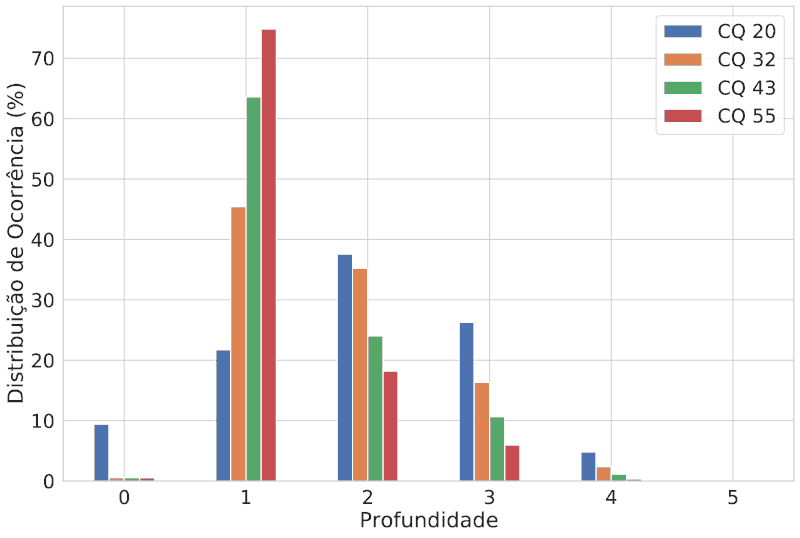
\includegraphics[width=0.75\textwidth]{FIGURES/fig_16.png}
    \caption{Média de distribuição das profundidades da árvore de particionamento do AV1. Fonte: Elaborada pelo autor.}
    \label{fig:16}
\end{figure}

Outra constatação a partir da Figura \ref{fig:16} é a relativa ausência de blocos 4$\times$4, que representam uma área média inferior a 0,3\% dos vídeos HD1080 utilizados nos experimentos. O mesmo pode ser observado com a profundidade 0, que ocupa uma área média inferior a 1\% em quase todos os experimentos realizados com diferentes níveis de quantização, exceto no caso da quantização configurada com CQ 20, onde a área de emprego da profundidade 0 é de 9\%. Essa observação contraria a expectativa de que vídeos codificados com menores parâmetros de quantização tendem a apresentar mais particionamentos; os resultados mostram que neste caso foram utilizados blocos maiores na codificação.

Em complemento à análise de distribuição de profundidades, é importante avaliar também o índice de utilização do modo de particionamento \textit{SPLIT} para cada profundidade da árvore. Essa informação é particularmente útil para definir quais profundidades são mais utilizadas e, consequentemente, quais são os particionamentos que, caso forçados ou evitados, têm potencial de causar maior impacto na eficiência de codificação do software do AV1. Utilizando os mesmos vídeos do experimento apresentado na Figura \ref{fig:16}, a Figura \ref{fig:17} mostra a taxa de uso do modo \textit{SPLIT} para cada profundidade e para cada nível de quantização considerado nos experimentos apresentados nesta tese. Na Figura \ref{fig:17}, os dados estão distribuídos de acordo com duas escolhas: o codificador decidiu pelo bloco naquele nível de profundidade (não-\textit{SPLIT}, em laranja) ou decidiu por subparticionar o bloco (\textit{SPLIT}, em azul). Em cada profundidade considerada (eixo x) o somatório de casos \textit{SPLIT} e não-\textit{SPLIT} é igual ao total de casos \textit{SPLIT} da profundidade anterior. No topo de cada coluna, encontra-se destacado o valor proporcional do modo \textit{SPLIT} (em azul) para aquela profundidade. Desta forma, torna-se possível identificar a probabilidade de ocorrência de particionamentos em cada profundidade e, ao mesmo tempo, identificar quais profundidades são utilizadas, complementando a Figura \ref{fig:16}. Por exemplo, na profundidade 2 (blocos 32$\times$32), considerando uma codificação com CQ 20, o codificador \textit{libaom} opta por subparticionar o bloco em blocos menores em 45,46\% das vezes. Quando processa blocos em profundidade 4, considerando o mesmo CQ 20, em apenas 4,11\% das vezes o codificador opta por subparticionar em blocos menores na profundidade 5.

\begin{figure}
    \centering
    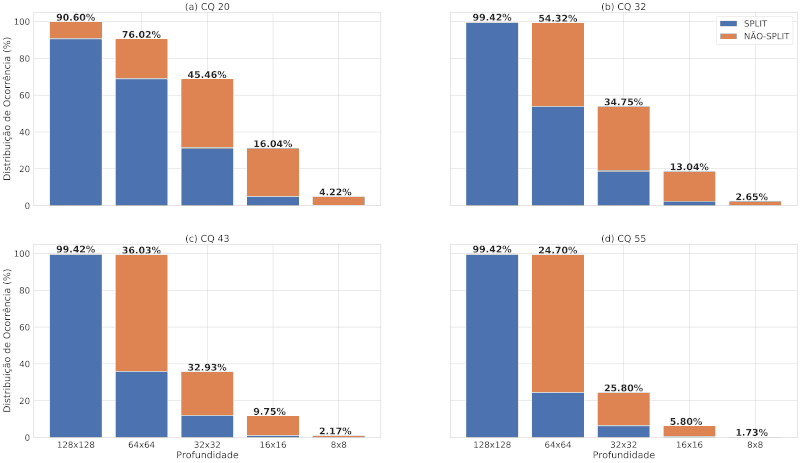
\includegraphics[width=\textwidth]{FIGURES/fig_17.png}
    \caption{Probabilidade do subparticionamento em modo \textit{SPLIT} para cada nível da árvore de particionamento do AV1, em CQs (a) 20, (b) 32, (c) 43 e (d) 55. Fonte: Elaborada pelo autor.}
    \label{fig:17}
\end{figure}

Evidenciamos neste capítulo que a escolha de particionamentos e de tamanhos de blocos influencia consideravelmente o custo computacional do software de referência do AV1 e também a sua eficiência de codificação. Portanto, uma das tarefas essenciais de um codificador ou transcodificador rápido, quando baseado em escolhas de particionamentos, é identificar a melhor combinação de blocos sem a necessidade de realizar um grande número de testes. Nesse sentido, o capítulo \ref{cap:6} contempla as primeiras soluções desenvolvidas no escopo desta tese, que envolvem transcodificadores rápidos por heurísticas baseados em análises estatísticas. No capítulo \ref{cap:7}, apresentamos a proposta de transcodificador rápido baseado no reaproveitamento de estruturas de particionamento com uso de modelos preditivos gerados por algoritmos de aprendizado de máquina, aplicados a diversos transcodificadores.
